\question{Особенности эмиссии электронов из термоэмиссионного катода на высоких
  частотах}

Пусть между анодом и катодом приложено некоторое напряжение
\[
  U_a = U_{a0}\sin\omega t + U_0.
\]

Пренебрегая начальными тепловыми скоростями электронов \( v_0 = 0 \), можно
считать, что величина тока эмиссии регулируется условием равенства нулю
напряженности электрического поля на катоде \( E(0) = 0 \).

Напряженность электрического поля складывается из напряженности электрического
поля, определяемой потенциалом на аноде, и из напряженности, определяемой
пространственным зарядом:
\[
  E = E_U + E_\text{пз}.
\]

Тогда плотность тока эмиссии с катода
\[
  j = \rho v = \rho\der{z}{t} = \Ez\pder{E}{z}\der{z}{t} = \Ez\pder{E}{t} =
    \Ez\pder{E_U}{t} + \Ez\pder{E_\text{пз}}{t} = j_\text{вч} + j_\text{Л}.
\]

При отсутствии высокочастотного поля эта плотность тока, очевидно, должна быть
равна плотности тока, описываемой законом Ленгмюра:
\[
  j_\text{Л} = \Ez\pder{E_\text{пз}}{t} = PU_a^{3 / 2}.
\]

Подставляя \( U_a \), получим:
\[
  j_\text{Л} = P\big( U_{a0}\sin\omega t + U_0 \big)^{3 / 2}.
\]

Пусть расстояние между анодом и катодом равно \( d \). Поскольку система
является плоской, то \( E_U = U_a / d \). Тогда
\[
  j_\text{вч} = \Ez\pder{E_U}{t} = \frac{\Ez}{d}\pder{U_a}{t} = \frac{\Ez}{d}
    U_{a0}\omega\cos\omega t.
\]

Таким образом, полный ток, эмитируемый с катода:
\[
  j = \frac{E_z}{d} U_{a0}\omega\cos\omega t +
    P\big( U_{a0}\sin\omega t + U_0 \big)^{3 / 2}.
\]

В зависимости от соотношения между \( U_0 \) и \( U_{a0} \) может наблюдаться
три различных ситуации.

\begin{figure}[h!]
  \center
%  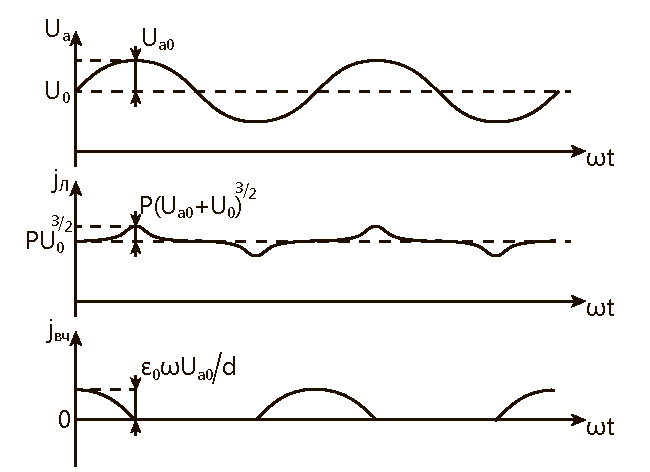
\includegraphics[width=.45\textwidth]{26_U0_g_Ua} \hspace{1em}
%  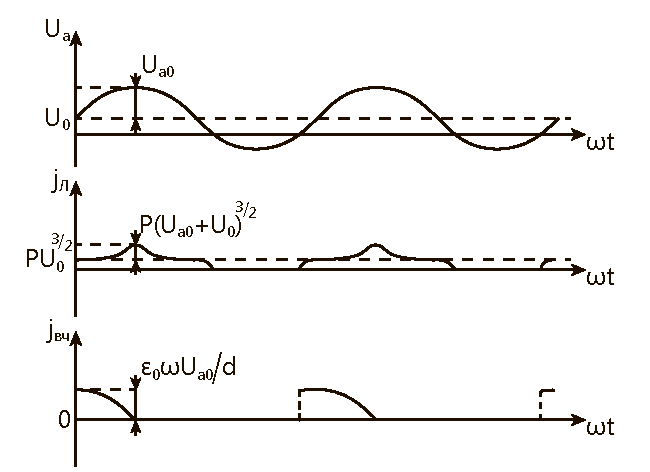
\includegraphics[width=.45\textwidth]{26_U0_g_0_l_Ua} \\
  \parbox{.45\textwidth}{\caption{Изменение \( U_a \), \( j_\text{Л} \) и
    \( j_\text{вч} \) при \( U_0 / U_{a0} > 1 \)}
    \label{pic26U0gUa}} \hspace{1em}
  \parbox{.45\textwidth}{\caption{Изменение \( U_a \), \( j_\text{Л} \) и
    \( j_\text{вч} \) при \( 0 < U_0 / U_{a0} < 1 \)}
    \label{pic26U0g0lUa}}
\end{figure}

\begin{enumerate}
  \item Случай \( U_0 / U_{a0} > 1 \). Тогда \( U_a \) всегда больше
    нуля и эмиссия с катода происходит во все моменты времени
    (рис.~\pic{26U0gUa}).

  \item Случай \( 0 < U_0 / U_{a0} < 1 \). В этой ситуации эмиссия может иметь
    место только в том интервале времени, когда мгновенное напряжение на аноде
    положительно, то есть когда \( \sin\omega t + U_0 / U_{a0} > 0 \)
    (рис.~\pic{26U0g0lUa}).

  \item Случай \( -1 < U_0 / U_{a0} < 0 \). В этой ситуации эмиссия также может
    иметь место только в том интервале времени, когда мгновенное напряжение на
    аноде положительно, то есть когда \( \sin\omega t > U_0 / U_{a0} \)
    (рис.~\pic{26U0l0}).
\end{enumerate}
  
Момент начала эмиссии \( t_0 \):
\begin{equation}
  U_{a0}\sin\omega t_0 + U_0 = 0, \quad
    t_0 = \frac{1}{\omega}\arcsin\left( -\frac{U_0}{U_{a0}} \right).
  \label{eq26t0}
\end{equation}

\begin{figure}[t!]
  \center
%  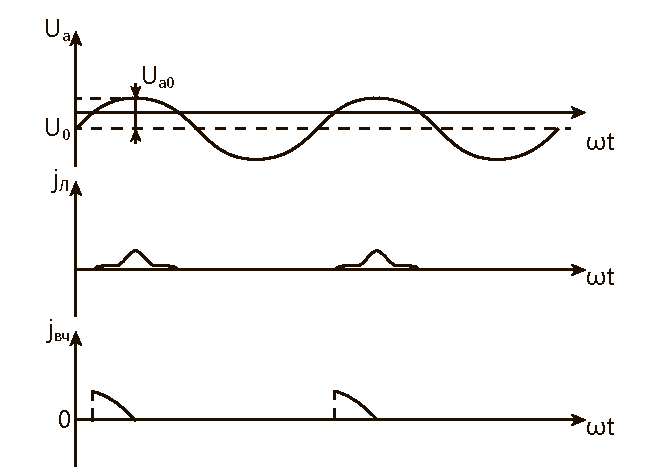
\includegraphics[width=.45\textwidth]{26_U0_l_0} \\
  \caption{Изменение \( U_a \), \( j_\text{Л} \) и \( j_\text{вч} \) при
    \( -1 < U_0 / U_{a0} < 0 \)}
  \label{pic26U0l0}
\end{figure}

Определим граничную частоту, после превышения которой будет необходимо
учитывать волновые эффекты.
\[
  j_{\text{Л}_{\max}} = P\big( U_{a0} - U_0 \big)^{3 / 2}; \quad
    j_{\text{вч}_{\max}} = \frac{\Ez}{d}U_{a0}\omega\cos\omega t_0 =
    \frac{\Ez\omega}{d}U_{a0}\sqrt{1 - \sin^2\omega t_0} =
    \frac{\Ez\omega}{d}\sqrt{U_{a0}^2 - U_0^2}.
\]

Тогда \( j_{\text{вч}_{\max}} / j_{\text{Л}_{\max}} = 1 \):
\[
  \frac{\Ez\omega\sqrt{U_{a0}^2 - U_0^2}}
    {dP\big( U_{a0} - U_0 \big)^{3 / 2}} = 1, \quad\text{или}\quad
    \frac{\Ez\omega\sqrt{U_{a0} + U_0}}
    {dP\big( U_{a0} - U_0 \big)} = 1;
\]
а для частоты
\[
 \omega_\text{г} = \frac{dP\big( U_{a0} - U_0 \big)}{\Ez\sqrt{U_{a0} + U_0}}.
\]
